\chapter{Numerics governing the atmospheric flows} \label{cha:NUM}
\section{Wind}
Wind is the movement of air relative to the Earth's surface, driven by the uneven heating of the atmosphere by solar radiation. This uneven heating creates pressure differences, which in turn cause air to move from high-pressure areas to low-pressure areas. The Earth's rotation and surface features further influence wind patterns, leading to complex and dynamic atmospheric flows. Wind plays a crucial role in various natural processes and is a key resource for renewable energy generation, particularly in wind turbines. 

\begin{figure}[ht]
    \centering
    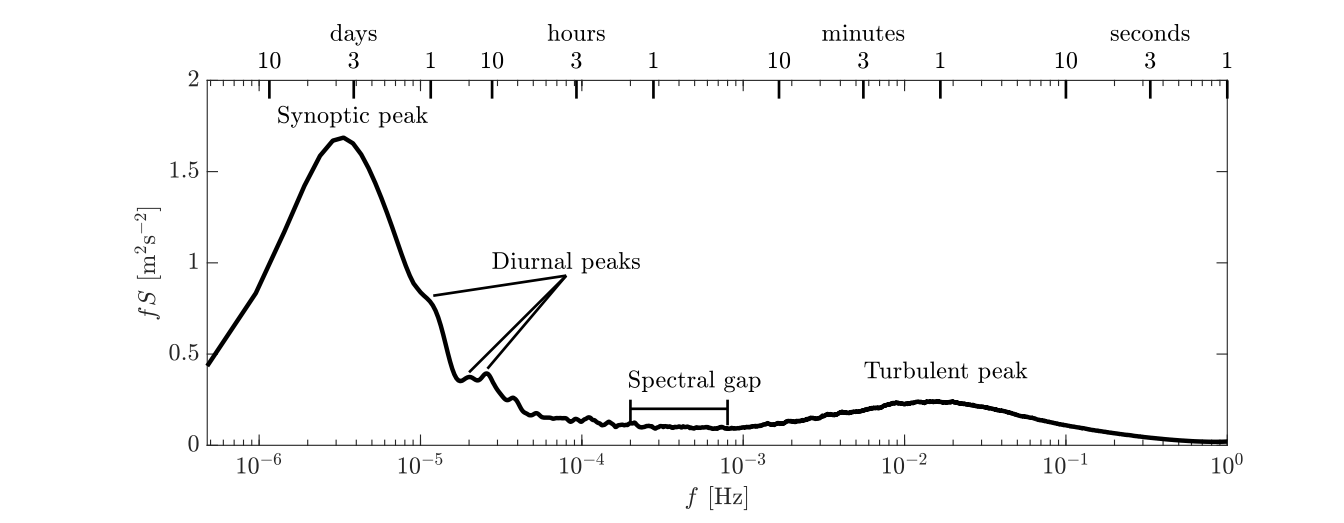
\includegraphics[width=\textwidth]{Figures/WindSpectra.png}
    \caption{Wind spectrum illustrating the distribution of energy across different frequencies at Bremerhaven measured by a cup anemometer
    at the height of 44 m \cite{Rettenmeier2013}.}
    \label{fig:windspectrum}
\end{figure}
As shown in Figure~\ref{fig:windspectrum}, the horizontal wind speed spectrum illustrates the distribution of energy across different frequencies. The synoptic peak is largely influenced by large-scale weather systems, while diurnal peaks arise from daily temperature variations between land and sea due to the day-night cycle. Between approximately 10 minutes and 1 hour, wind fluctuations tend to be minimal under normal conditions; this region is commonly referred to as the spectral gap. At higher frequencies—those associated with minute-scale variations—a distinct peak appears, which is linked to atmospheric turbulence.

In the context of modern wind turbines, high-frequency wind fluctuations are particularly significant because they often align with the natural frequencies of turbine structures, thereby contributing to fatigue loads. Conversely, low-frequency components of the spectrum are more relevant for understanding variations in power output and maintaining grid stability \cite{kosovic2025}. Due to the spectral gap, wind turbine design typically focuses on characterizing turbulent and mean wind components over time intervals of 10 to 30 minutes. Using longer intervals risks incorporating diurnal variations, which have little influence on turbine loading.

\subsection{Kaimal Spectrum}
The Kaimal spectrum is a widely used model to represent the energy distribution of turbulence in the atmospheric boundary layer. It provides a mathematical representation of the wind spectrum, particularly for horizontal wind speed fluctuations. The Kaimal spectrum is defined as:

\begin{equation}
S_u(f) = \frac{\sigma_u^2 L_u}{U} \frac{4fL_u/U}{\left(1 + 6fL_u/U\right)^{5/3}}
\end{equation}

where:
\begin{itemize}
    \item $S_u(f)$ is the power spectral density of the longitudinal wind speed fluctuations at frequency $f$,$\sigma_u$ is the standard deviation of the longitudinal wind speed fluctuations, $L_u$ is the integral length scale of turbulence in the longitudinal direction, $U$ is the mean wind speed, $f$ is the frequency.
\end{itemize}

The Kaimal spectrum captures the energy distribution across different frequencies, with the following characteristics:
\begin{itemize}
    \item At low frequencies, the spectrum exhibits a $f^{-1}$ behavior, indicating that large-scale eddies dominate the energy.
    \item At high frequencies, the spectrum follows a $f^{-5/3}$ decay, consistent with Kolmogorov's theory of turbulence for the inertial subrange.
\end{itemize}

This spectrum is particularly useful for wind turbine design, as it provides insights into the turbulent energy content at different scales, which directly impacts turbine loading and performance. Figure~\ref{fig:windspectrum} illustrates how the Kaimal spectrum aligns with the observed wind spectrum, highlighting its relevance in characterizing atmospheric turbulence.

The consistency between wind modeling approaches and actual measurement data supports the common practice of separating wind into mean components and turbulence spectra. Consequently, wind turbine simulations are typically conducted as follows: 

First, a series of turbulent wind fields—each 10 minutes long—are generated based on turbulence and vertical wind shear models for various mean wind speeds. According to \cite{iec61400},running at least six simulations per mean wind speed, spaced at 2~m/s intervals from cut-in to cut-out speeds, is recommended to ensure statistically reliable results. Second, the wind speed distribution is modeled using a probability density function, which is then used to extrapolate and weight performance metrics such as power output, pitch activity, and structural loads over the turbine's operational lifetime.

The wind fields used in aero-elastic simulations are time series of three-dimensional wind velocity vectors defined at discrete points on a vertical, stationary, two-dimensional grid. In this study, wind fields are generated using \texttt{TurbSim}~\cite{turbsim09}, which applies a rectangular grid layout. These wind fields are then used in \texttt{FAST} for aero-elastic simulations, where they are interpolated along the rotating blades to compute aerodynamic forces and moments using the Blade Element Momentum (BEM) method, as described in Section \ref{sec:bem_theory}. 

Although the rotor plane can shift longitudinally due to nacelle motion or blade deflection, the wind field imported into \texttt{FAST} remains fixed and does not account for such movements.


The Kaimal spectrum, widely used in wind turbine load analysis, has notable limitations: it captures only second-order turbulence statistics, assumes Gaussian-distributed wind fluctuations (underestimating extreme events), and fails to represent intermittent, gusty features or heavy-tailed distributions observed in real atmospheric inflows. These shortcomings can lead to inaccuracies in predicting alternating loads on turbine components and discrepancies in torque statistics compared to real atmospheric data, potentially causing design and operational errors \cite{Mucke2011}.

A numerical flow model like Large Eddy Simulation(LES) is important compared to the Kaimal spectrum because it provides a more realistic and detailed representation of atmospheric turbulence. While the Kaimal model is limited to basic statistical properties and assumes Gaussian, stationary turbulence, numerical models solve the actual fluid dynamics equations, capturing complex and non-Gaussian features like gusts, ramps, and coherent structures. This allows for better prediction of loads and fatigue on wind turbines, especially in turbulent and complex terrains. Unlike the Kaimal model, numerical simulations offer spatial and temporal coherence, making them more suitable for modern applications like wake modeling, advanced turbine control, and site-specific assessments. \cite{Doubrawa2019}


\section{The Governing Equations of flow of motion}
\subsection{Navier-Stokes equations}
The motion of viscous fluids (e.g. the air flow over wind turbine blades) can be described by
means of the Navier-Stokes equations \cite{NSeqn}, which are based on the conservation of mass, momentum
and energy. The energy equation is disregarded in this thesis, since it is only required for
compressible flows (compressible effects are negligible in wind turbines since Ma < 0.3). The
Navier-Stokes equations assuming constant density can be written in differential, scalar form
as:
\begin{tcolorbox}[colback=blue!5!white, colframe=blue!75!black]
    \textbf{Navier-Stokes equations:}
    \newline
    \textbf{Conservation of Mass:}
    The conservation of mass, also known as the continuity equation, ensures that mass is neither
    created nor destroyed. For an incompressible fluid, this is expressed as:
    \begin{equation}
    \nabla \cdot \mathbf{u} = 0
    \end{equation}
    where $\mathbf{u}$ is the velocity vector of the fluid.
    
    \textbf{Conservation of Momentum:}
    The conservation of momentum describes how the velocity of the fluid changes due to forces acting on it. For an incompressible fluid, the Navier-Stokes momentum equation is:
    \begin{equation}
    \rho \left( \frac{\partial \mathbf{u}}{\partial t} + \mathbf{u} \cdot \nabla \mathbf{u} \right) = -\nabla p + \mu \nabla^2 \mathbf{u} + \mathbf{f}
    \end{equation}
    where:
    \begin{itemize}
        \item $\rho$ is the fluid density (assumed constant), $\mathbf{u}$ is the velocity vector, $p$ is the pressure, $\mu$ is the dynamic viscosity, $\mathbf{f}$ represents external body forces (e.g., gravity, coriolis forces).
    \end{itemize}
    For detailed information on the Navier-Stokes equations, refer to \cite{NSeqn}
\end{tcolorbox}



\subsection{Turbulence Modeling}

Turbulence modeling is essential for understanding and simulating fluid flows at high Reynolds numbers. At low Reynolds numbers, the flow is laminar, with smooth and orderly motion. However, at high Reynolds numbers, the flow becomes turbulent, characterized by chaotic velocity and pressure fluctuations. These fluctuations result in increased mixing and diffusion of mass, momentum, and energy.

Turbulent flows exhibit an energy cascade, where large eddies extract energy from the mean flow and transfer it to smaller eddies through vortex stretching. This process continues until the smallest eddies dissipate energy into heat due to viscous effects.

The transition to turbulence is often triggered by flow instabilities in sheared flows. These instabilities amplify, leading to the formation of rotational structures and fully turbulent flows. To simulate turbulent flows, various strategies are employed, including Direct Numerical Simulation (DNS), Reynolds-Averaged Navier-Stokes (RANS), and Large Eddy Simulation (LES), each with its own trade-offs in accuracy and computational cost.

\subsection{Direct Numerical Simulation (DNS) and its limitations:}
Direct Numerical Simulation (DNS) involves solving the Navier-Stokes equations without any turbulence modeling, 
resolving all scales of motion down to the smallest eddies. While DNS provides highly accurate results, 
it is computationally prohibitive for most practical engineering applications, including wind turbines.

The computational cost of DNS scales with the Reynolds number ($Re$) as $Re^{3}$ to $Re^{3.5}$, 
due to the need to resolve the smallest turbulent scales. For wind turbines, the Reynolds number is typically in the range of $10^6$ to $10^7$, 
making DNS infeasible. Furthermore, the use of DNS also requires very accurate, low-dissipative numerical schemes
\cite{mocket2009}. This makes this type of simulation unsuitable for most technical applications,
especially for high Reynolds number flows. According to \cite{spalart2000}, the computational
power required for simulating an aircraft by means of CFD will not be readily available before
the year 2080. However, DNS is already used for performing basic turbulence research at low
Reynolds numbers 
Additionally, the large physical domain of wind turbine simulations, which includes the rotor blades and the surrounding atmospheric boundary layer, 
\subsection{Reynolds-Averaged Navier-Stokes (RANS) Equations}
To address the computational challenges of Direct Numerical Simulation (DNS), the Reynolds-Averaged Navier-Stokes (RANS) equations are commonly used. The RANS approach involves decomposing the instantaneous velocity and pressure fields into mean and fluctuating components:

\begin{equation}
\mathbf{u} = \overline{\mathbf{u}} + \mathbf{u}'
\end{equation}
\begin{equation}
p = \overline{p} + p'
\end{equation}

where:
\begin{itemize}
    \item $\overline{\mathbf{u}}$ and $\overline{p}$ are the mean velocity and pressure fields, $\mathbf{u}'$ and $p'$ are the fluctuating components of velocity and pressure.
\end{itemize}

Substituting these decompositions into the Navier-Stokes equations and applying a time-averaging operation results in the RANS equations:
\textbf{Reynolds-Averaged Navier-Stokes (RANS) Equations:}

\textbf{Conservation of Mass:}
\begin{equation}
\nabla \cdot \overline{\mathbf{u}} = 0
\end{equation}

\textbf{Conservation of Momentum:}
\begin{equation}
\rho \left( \frac{\partial \overline{\mathbf{u}}}{\partial t} + \overline{\mathbf{u}} \cdot \nabla \overline{\mathbf{u}} \right) = -\nabla \overline{p} + \mu \nabla^2 \overline{\mathbf{u}} - \nabla \cdot \overline{\mathbf{u}' \mathbf{u}'}
\end{equation}

Here, the Reynolds stress tensor $\overline{\mathbf{u}' \mathbf{u}'}$ is defined as:
\begin{equation}
\overline{\mathbf{u}' \mathbf{u}'} = 
\begin{bmatrix}
\overline{u'^2} & \overline{u'v'} & \overline{u'w'} \\
\overline{v'u'} & \overline{v'^2} & \overline{v'w'} \\
\overline{w'u'} & \overline{w'v'} & \overline{w'^2}
\end{bmatrix}
\end{equation}

The term $\overline{\mathbf{u}' \mathbf{u}'}$ represents the Reynolds stresses, 
which account for the effects of turbulence on the mean flow. 
These stresses introduce additional unknowns, making the system of equations unclosed. 
To close the RANS equations, turbulence models such as the $k$-$\epsilon$ or $k$-$\omega$ models are used to approximate the Reynolds stresses.

RANS has the advantage of being computationally efficient and widely validated, making it suitable for many engineering applications where time-averaged solutions are sufficient.
However, its reliance on turbulence models introduces approximations, which can reduce accuracy for flows with strong unsteadiness, separation, or complex turbulence structures.

\subsection{Large Eddy Simulation (LES)}
Large Eddy Simulation (LES) is a numerical technique used to simulate turbulent flows by resolving the large-scale turbulent structures 
while modeling the effects of smaller, sub-grid scale (SGS) motions. LES bridges the gap between Direct Numerical Simulation (DNS) 
and Reynolds-Averaged Navier-Stokes (RANS) by providing a balance between computational cost and accuracy.

In atmospheric flows Large Scale eddies contain more energy and transport moreeffectively the 
momentum and scalars than the small scale eddies\cite{spalart2000}. Thats why putting
more computational effort on the large scale eddies is more efficient than putting it on the small scale eddies and it 
does not severely comprimise simulation accuracy. Furthermore, modelling the small scale turbulence is comparatively simple because of
its isotropic, homogeneous and universal characteristics (in opposition to the anisotropic and
anisotropic problem-specific characteristics of large scale turbulence).
The LES approach involves applying a spatial filtering operation to the Navier-Stokes equations,
which separates the flow field into resolved (large-scale) and unresolved (small-scale) components.
The filtering operation is defined as: 
\begin{equation}
\overline{\phi}(\mathbf{x}, t) = \int_V \phi(\mathbf{x}', t) G(\mathbf{x} - \mathbf{x}') d\mathbf{x}'
\end{equation}
where:
\begin{itemize}
    \item $\phi$ is a flow variable (e.g., velocity, pressure), $G$ is the filter function, which determines the scale of the resolved motions, $V$ is the volume of the computational domain.
\end{itemize}

Different types of filter exist, but all of them have in common the
usage of a length scale $\Delta$ which is the filter width. The filter width
is the characteristic length scale of the large eddies that are resolved in the simulation.
The filter function $G$ is typically chosen to be a Gaussian or box filter,
which allows for the separation of large and small scales. The filter width $\Delta$ is a critical parameter that determines the scale of the resolved motions in the simulation.

Applying the filtering operation to the Navier-Stokes equations results in the filtered equations of motion:

\textbf{Filtered Conservation of Mass:}
\begin{equation}
\nabla \cdot \overline{\mathbf{u}} = 0
\end{equation}

\textbf{Filtered Conservation of Momentum:}
\begin{equation}
\rho \left( \frac{\partial \overline{\mathbf{u}}}{\partial t} + \overline{\mathbf{u}} \cdot \nabla \overline{\mathbf{u}} \right) = -\nabla \overline{p} + \mu \nabla^2 \overline{\mathbf{u}} - \nabla \cdot \tau_{SGS}
\end{equation}
where $\tau_{SGS}$ is the sub-grid scale stress tensor, defined as:
\begin{subequations}
    \begin{equation}
    \tau_{SGS} = \overline{\mathbf{u} \mathbf{u}} - \overline{\mathbf{u}} \, \overline{\mathbf{u}}
    \end{equation}
\end{subequations}
    

The sub-grid scale stress tensor $\tau_{SGS}$ represents the effects of the unresolved small-scale motions on the resolved large-scale motions. To close the LES equations, $\tau_{SGS}$ must be modeled using a sub-grid scale model.

The sub-grid scale (SGS) stress tensor $\boldsymbol{\tau}_{\mathrm{SGS}}$ represents the effects of unresolved small-scale motions on the resolved large-scale motions. To close the LES equations, $\boldsymbol{\tau}_{\mathrm{SGS}}$ must be modeled using a sub-grid scale model.

\begin{tcolorbox}[colback=blue!5!white, colframe=blue!75!black]
\textbf{Sub-Grid Scale Models:}

Two widely used models to approximate $\boldsymbol{\tau}_{\mathrm{SGS}}$ are:

\vspace{1mm}
\textbf{Smagorinsky Model:} 
The Smagorinsky model assumes that the SGS stresses are proportional to the strain rate of the resolved flow:
\begin{equation}
\boldsymbol{\tau}_{\mathrm{SGS}} = -2 \nu_t \mathbf{S}
\end{equation}
where:
\begin{itemize}
    \item $\nu_t = (C_s \Delta)^2 |\mathbf{S}|$ is the eddy viscosity,
    \item $C_s$ is the Smagorinsky constant (typically $C_s \approx 0.1$),
    \item $\Delta$ is the filter width,
    \item $\mathbf{S}$ is the strain-rate tensor, defined as $\mathbf{S} = \frac{1}{2} \left( \nabla \overline{\mathbf{u}} + \nabla \overline{\mathbf{u}}^{\mathrm{T}} \right)$.
\end{itemize}

\vspace{2mm}
\textbf{Dynamic Smagorinsky Model:} 
This model improves upon the standard Smagorinsky model by dynamically computing the coefficient $C_s$ based on the local flow conditions. 

A second filtering operation, called the \textit{test filter}, is applied and the Germano identity is used to compute $C_s$:
\begin{itemize}
    \item This makes the model adaptive to local turbulence structures,
    \item It improves accuracy especially in complex and inhomogeneous flows.
\end{itemize}
\end{tcolorbox}

Large-eddy simulation (LES) provides a detailed representation of turbulent flows by resolving energy-containing large eddies while modeling the dissipative smaller scales. It is widely used in engineering and scientific applications where direct numerical simulation (DNS) is computationally prohibitive and Reynolds-averaged Navier–Stokes (RANS) methods lack sufficient fidelity.

In the present work, the large-eddy simulation tool \macro{PALM} \cite{maronga2015}, developed at the Institute for Meteorology and Climatology (IMUK) of Leibniz University Hannover, is employed.


LES provides a detailed representation of turbulent flows, capturing the energy-containing large eddies while modeling the dissipative small scales. It is widely used in engineering and scientific applications where DNS is computationally infeasible, and RANS lacks sufficient accuracy. In the present work the
large-eddy simulation (LES) tool \macro{PALM} \cite{maronga2015}, developed at the Institute for Meteorology and
Climatology (IMUK) of Leibniz University Hannover is used. 

The \macro{PALM model} is built upon the non-hydrostatic, filtered, incompressible Navier–Stokes equations, formulated using the Boussinesq approximation. An anelastic approximation is also available as an option for simulating deep convection. By default, PALM solves for at least six prognostic variables: the three velocity components ($u$, $v$, $w$) on a Cartesian grid, the potential temperature ($\theta$), the water vapor mixing ratio ($q_v$), and optionally a passive scalar ($s$). Additionally, a prognostic equation is solved either for the subgrid-scale turbulent kinetic energy (SGS-TKE, $e$) in large-eddy simulation (LES) mode—used by default—or for the total turbulent kinetic energy in Reynolds-averaged Navier–Stokes (RANS) model.

In LES mode, the filtering operation introduces four subgrid-scale (SGS) covariance terms, which are parameterized using a 1.5-order turbulence closure following Deardorff (1980). PALM employs a modified version of the closure schemes proposed by Moeng and Wyngaard (1988) and Saiki et al. (2000). This closure assumes that the energy transport by SGS eddies is proportional to the local gradients of the resolved flow variables.

A comprehensive description of PALM and its functionalities can be found in the official PALM documentation and related publications\cite{maronga2015} \cite{raasch2001}.

\chapter{Numberics governing Aeroelastic Simulation of a Wind Turbine}
\section{Aeroelastic Simulation of a Wind Turbine}

\subsection{Blade Element Momentum (BEM) Theory} 
\label{sec:bem_theory}

Wind turbines are commonly modeled using aeroelastic simulation tools, which provide reliable system-level accuracy and are widely used in certification procedures. The Blade Element Momentum (BEM) theory is a widely used method for analyzing the aerodynamic performance of wind turbine blades. It combines two fundamental principles: the blade element theory and the momentum theory. These equations can be solved iteratively under the assumption that aerodynamic interactions between blade elements are negligible \cite{ingram2011blade}. The first approach, known as Momentum Theory, is based on applying force and momentum balance to an annular streamtube. The second, Blade Element Theory, calculates lift and drag forces at discrete sections along the blade.
\subsubsection{Momentum Theory}
Consider a streamtube surrounding a wind turbine rotor,
\begin{figure}[ht]
    \centering
    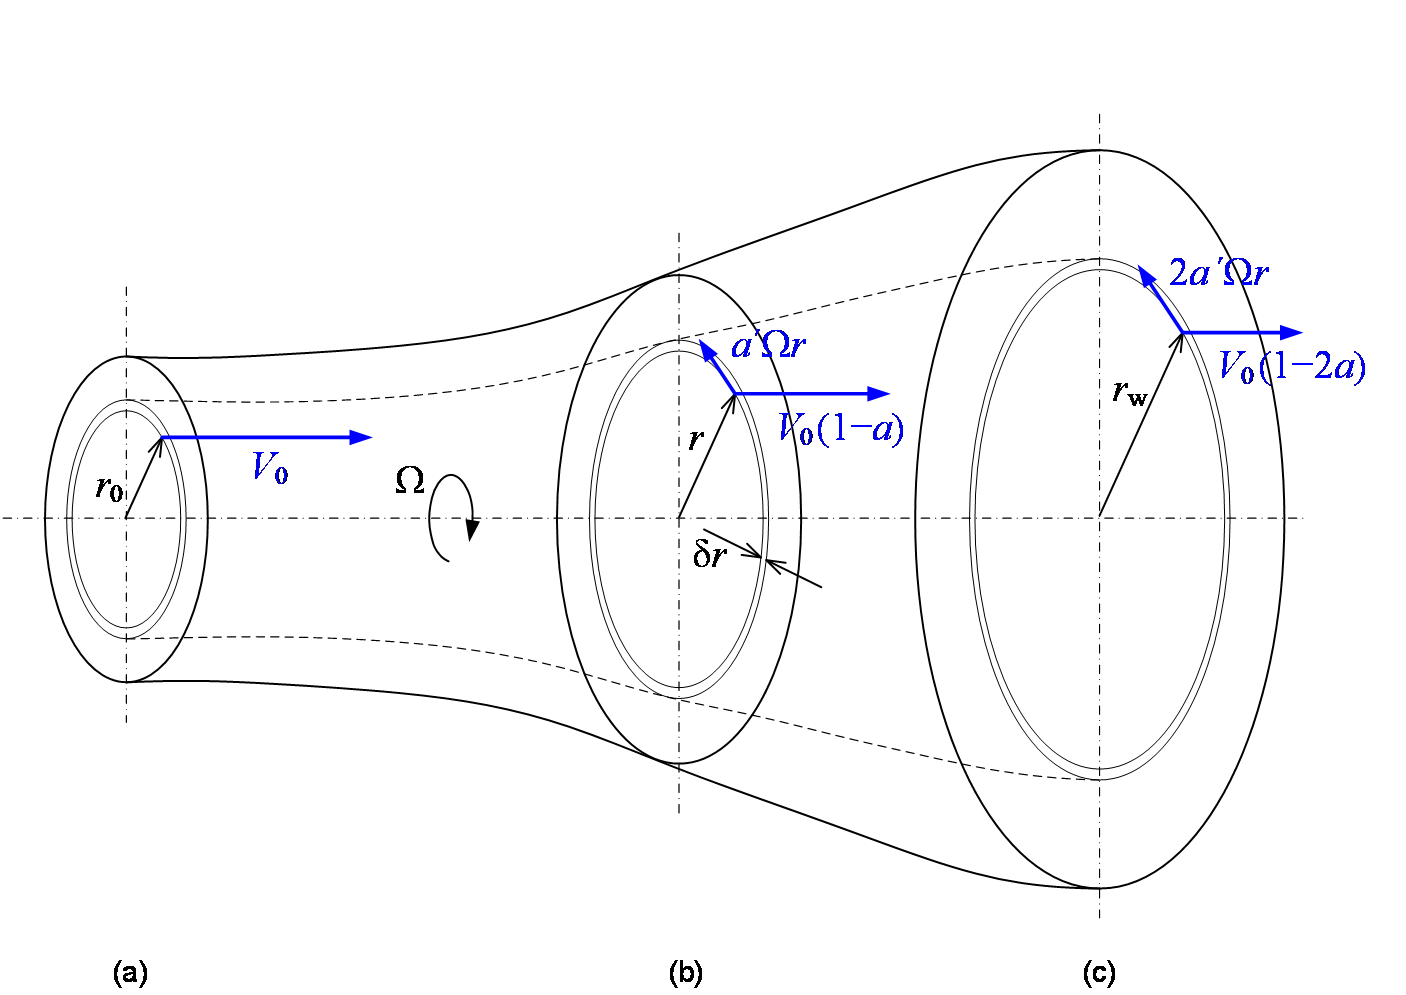
\includegraphics[width=\textwidth]{Figures/aerodynamics_streamtube.png}
    \caption{Streamtube around a wind turbine rotor.}
    \label{fig:streamtube}
\end{figure}


The axial force $dF_x$ and torque $dT$ on an annular element of a wind turbine rotor can be expressed as:

Axial Force:
\begin{equation}
dF_x = 4\pi \rho V_1^2 a(1 - a) r \, dr
\end{equation}

Tangential Force:
\begin{equation}
dT = 4\pi \rho a' (1 - a) \Omega V_1 r^3 \, dr
\end{equation}

Here, $a$ is the axial induction factor, $a'$ is the angular induction factor, $\rho$ is the air density, $V_1$ is the free-stream wind speed, $\Omega$ is the angular velocity of the rotor, $r$ is the radial position, and $dr$ is the thickness of the annular element. For detailed information on the BEM theory and its derivations, refer to \cite{ingram2011blade}.
\subsubsection{Blade Element Theory}
The blade element theory calculates the aerodynamic forces acting on a small element of the rotor blade. The lift and drag forces can be expressed as:
\begin{equation}
dF_L = \frac{1}{2} \rho V^2 C_L dA
\end{equation}
\begin{equation}
dF_D = \frac{1}{2} \rho V^2 C_D dA
\end{equation}

where:
\begin{itemize}
    \item $dF_L$ is the lift force, $dF_D$ is the drag force, $\rho$ is the air density, $V$ is the relative wind speed at the blade element, $C_L$ and $C_D$ are the lift and drag coefficients, respectively, and $dA$ is the area of the blade element.
\end{itemize}
The lift and drag coefficients are functions of the angle of attack ($\alpha$) and can be obtained from experimental data or empirical models. The angle of attack is defined as:
\begin{equation}
\alpha = \beta - \phi
\end{equation}
where:
\begin{itemize}
    \item $\beta$ is the pitch angle of the blade element, and $\phi$ is the angle between the relative wind direction and the chord line of the blade element.
\end{itemize}
The aerodynamic forces on a wind turbine blade segment depend on the lift and drag coefficients, $c_L(\alpha)$ and $c_D(\alpha)$, which vary with the angle of attack $\alpha$. The angle $\beta$ represents the inclination of the blade segment relative to the rotor plane, as illustrated in Figure~\ref{fig:blade_geometry}.

The differential aerodynamic thrust and torque on an annular ring can be expressed as:
\begin{align}
    dF_a &= n_B \left( dL_a \cos(\alpha + \beta) + dD_a \sin(\alpha + \beta) \right), \label{eq:thrust_force} \\
    dM_a &= n_B \left( dL_a \sin(\alpha + \beta) - dD_a \cos(\alpha + \beta) \right) r, \label{eq:torque}
\end{align}
where $n_B$ is the number of blades, $dL_a$ and $dD_a$ are the differential lift and drag forces, and $r$ is the radial position.
\begin{figure}[ht]
    \centering
    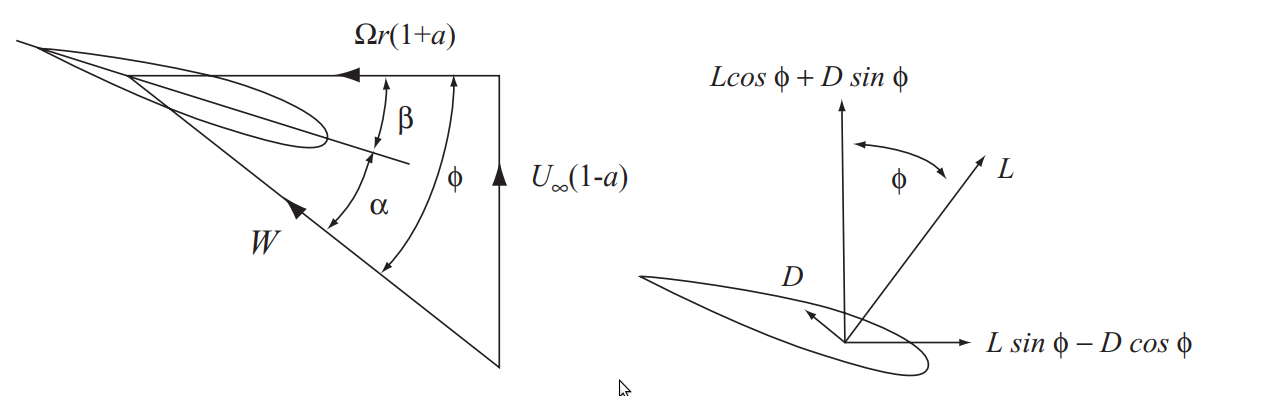
\includegraphics[width=\textwidth]{Figures/blade_element.png}
    \caption{Blade element velocities (left) and forces (right) \cite{burton2011}.}
    \label{fig:blade_geometry}
\end{figure}

From geometric considerations shown in Figure~\ref{fig:blade_geometry}, the inflow angle is given by:
\begin{equation}
    \tan(\alpha + \beta) = \frac{u_\infty(1 - a)}{\Omega r (1 + a)},
\end{equation}
and the relative inflow speed is:
\begin{equation}
    v_{\text{inflow}}^2 = \left( \Omega r (1 + a) \right)^2 + \left( u_1 (1 - a) \right)^2. \label{eq:inflow_speed}
\end{equation}

Equations~\eqref{eq:thrust_force} and~\eqref{eq:torque} are equated with the corresponding expressions from momentum theory to form a system of two nonlinear equations. The unknowns $a_{\text{ax}}$ (axial induction factor) and $a_{\text{an}}$ (angular induction factor) are then solved iteratively for each blade section, given known values of $u_1$, $\Omega$, $\rho$, $\beta$, $r$, $dr$, $c$, and the aerodynamic coefficients $c_L(\alpha)$ and $c_D(\alpha)$.
For detailed information on the Blade Element theory and its derivations, refer to \cite{ingram2011blade}.

The total aerodynamic thrust and torque are obtained by integrating $dF_a$ and $dM_a$ across all blade elements. The aerodynamic module of FAST implements these calculations along with empirical corrections such as tip and hub loss factors~\cite{fastV3}, enhancing the accuracy of the Blade Element Momentum (BEM) method.
         
\subsection{Structural Dynamics of Wind Turbines}

Wind turbine structural dynamics can be modeled using two main approaches: finite element (FE) models and modal analysis~\cite{bossanyi2010}. In practice, modal models with fewer Degrees of Freedom (DOFs) are often preferred due to their lower computational cost.

In this work, the FAST code is used to model the turbine structure. The structural equations are derived in a preprocessing step using \texttt{BModes}~\cite{bir2009}. The tower and blades are modeled as Euler-Bernoulli beams, which are discretized into multiple segments using finite element methods. This results in a system of nonlinear, coupled Ordinary Differential Equations (ODEs), capturing variations in mass, stiffness, and inertia along the structure.

These nonlinear equations are linearized, and an eigenvalue analysis is performed to extract the natural vibration modes. The resulting mode shapes $\mu_i(r)$, distributed mass, and stiffness properties are stored in input files for FAST. Each mode shape $\mu_i(r)$ is a polynomial in the radial position $r$ and is normalized such that $\mu_i(r_{\text{end}}) = 1$.

Assuming small deflections, a linear modal representation is used for blades and tower. For each mode $i$, the modal mass $m_i$, stiffness $k_i$, damping $c_i$, and external force $F_i$ are computed using:

\begin{align}
    m_i &= \sum_{j=1}^{n_S} m_j \mu_i^2(r_j), \label{eq:modal_mass} \\
    k_i &= \sum_{j=1}^{n_S} k_j \mu_i^2(r_j), \label{eq:modal_stiffness} \\
    c_i &= \frac{d_{s,i} k_i}{\pi f_{0,i}}, \quad f_{0,i} = \frac{1}{2\pi} \sqrt{\frac{k_i}{m_i}}, \label{eq:modal_damping} \\
    F_i &= \sum_{j=1}^{n_S} F_j \mu_i(r_j), \label{eq:modal_force}
\end{align}

where $d_{s,i}$ is the structural damping ratio, and $f_{0,i}$ is the natural frequency of mode $i$.

The equation of motion for a single mode is:

\begin{equation}
    m_i \ddot{q}_i + c_i \dot{q}_i + k_i q_i = F_i. \label{eq:single_mode_eom}
\end{equation}

\begin{figure}[ht]
    \centering
    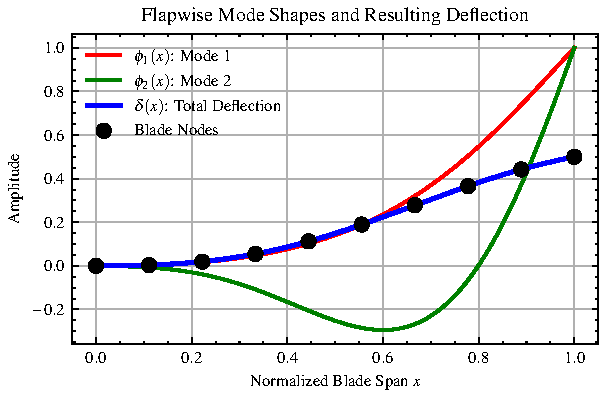
\includegraphics[width=\textwidth]{Figures/blade_modes.pdf}
    \caption{Blade mode shapes illustrating the first edgewise mode and the first two flapwise modes of a NREL 5 MW Turbine.}
    \label{fig:blade_mode_shapes}
\end{figure}

In FAST, each blade is modeled using the first edgewise mode and the first two flapwise modes. The tower is modeled with the first two modes in both fore-aft and side-to-side directions. Including rotor rotation, drive train torsion, and nacelle yaw, this results in a total of 16 DOFs for a three-bladed wind turbine.

The total deflection of a flexible component is reconstructed by superimposing all mode shapes weighted by the current modal amplitudes. The coupled equations of motion are derived using Kane’s method~\cite{kane1985}, which accounts for nonlinear interactions between structural and rotational DOFs. For example, tower motion depends on the instantaneous azimuthal positions of the blades. Rotor speed also affects mode frequencies due to centrifugal stiffening.

The complete system of equations is written in the general form:

\begin{equation}
    \mathbf{M}(\mathbf{q}, \mathbf{u}) \ddot{\mathbf{q}} + \mathbf{f}(\mathbf{q}, \dot{\mathbf{q}}, \mathbf{u}, \mathbf{d}) = 0, \label{eq:general_eom}
\end{equation}

where $\mathbf{q}$ is the vector of modal coordinates, $\mathbf{u}$ represents control inputs, and $\mathbf{d}$ includes external disturbances such as wind loads.

\section{Numerical Flow model of a Wind Turbine}
\subsection{The Actuator Line Model} 

The Actuator Line Model (ALM) is a numerical approach used to simulate the aerodynamic forces exerted by wind turbine blades on the surrounding flow field. In this model, the blades are represented as lines of discrete force elements rather than as solid surfaces. These force elements are distributed along the span of the blade and are computed based on the local flow conditions and the blade's aerodynamic properties. The ALM captures the unsteady aerodynamic interactions between the blades and the turbulent flow, making it suitable for high-fidelity simulations of wind turbine wakes and rotor dynamics. The forces are smoothed using a Gaussian kernel to avoid numerical instabilities and to account for the finite resolution of the computational grid. This smoothing ensures that the aerodynamic forces are distributed over a small region around the actuator line, rather than being concentrated at discrete points.

The ALM is computationally efficient compared to fully resolved blade simulations, as it eliminates the need to resolve the blade geometry explicitly. However, it requires accurate input data, such as airfoil characteristics and blade geometry, to ensure reliable results. The model is widely used in Large Eddy Simulations (LES) of wind farms, where it provides detailed insights into wake interactions and turbulence effects.
\subsection{The Actuator Disk Model} 
The Actuator Disk Model (ADM) is a simplified approach for simulating the aerodynamic effects of a wind turbine rotor on the flow field. In this model, the rotor is represented as a permeable disk that exerts a uniform or spatially varying force distribution on the incoming flow. The ADM is based on the principles of momentum theory and assumes that the rotor induces a pressure drop and velocity deficit in the flow, which are proportional to the thrust and power coefficients of the turbine. The ADM is computationally less demanding than the Actuator Line Model, as it does not require detailed blade geometry or airfoil data. It is particularly useful for large-scale simulations of wind farms, where the focus is on the overall flow dynamics rather than the detailed blade aerodynamics. However, the ADM lacks the ability to capture unsteady blade-wake interactions and the effects of blade-specific aerodynamic features. Despite these limitations, the ADM remains a valuable tool for studying wind farm performance, wake interactions, and optimization strategies in scenarios where computational resources are limited.
\subsection{The Actuator Sector Model} 


